%%%%%%%%%%%%%%%%%%%%%%%%%%%%%%%%%%%%%%%%%
% Imperial College London
% UKRI Centre for Doctoral Training in AI for Healthcare
% https://ai4health.io
%
% LaTeX Template
% Version 1.0 (22/10/19) Aldo Faisal
%%%%%%%%%%%%%%%%%%%%%%%%%%%%%%%%%%%%%%%%%
%----------------------------------------------------------------------------------------
%	PACKAGES AND OTHER DOCUMENT CONFIGURATIONS
%----------------------------------------------------------------------------------------
\documentclass[french]{report}
%encoding
%--------------------------------------
\usepackage[utf8]{inputenc}
\usepackage[T1]{fontenc}
%--------------------------------------

%French-specific commands
%--------------------------------------
\usepackage{babel}
\usepackage[autolanguage]{numprint}
%--------------------------------------

%Hyphenation rules
%--------------------------------------
\usepackage{hyphenat}
\hyphenation{mathéma-tiques récu-pérer}
%--------------------------------------
\usepackage{amssymb}
\usepackage{amsmath}
\usepackage{graphicx}
\usepackage{fancyhdr}
\usepackage{bm}
\usepackage{hyperref}
\usepackage{fancyhdr}
\usepackage{glossaries}
\usepackage{url}
\usepackage{indentfirst}
\makeatletter
\g@addto@macro{\UrlBreaks}{\UrlOrds}
\makeatother



\documentclass[a4paper,12pt]{article}
\usepackage[english]{babel}
\usepackage[latin1]{inputenc}
\usepackage{amsmath}
\usepackage{amssymb}
\usepackage{amsfonts}
\usepackage{graphicx}
\usepackage[colorinlistoftodos]{todonotes}
\usepackage[toc,page]{appendix}
\usepackage{geometry}
 \geometry{
 a4paper,
 total={170mm,257mm},
 left=20mm,
 top=20mm,
 }
 \usepackage{hyperref}
 \hypersetup{
    bookmarks=true,         % show bookmarks bar?
    unicode=false,          % non-Latin characters in Acrobat’s bookmarks
    pdftoolbar=true,        % show Acrobat’s toolbar?
    pdfmenubar=true,        % show Acrobat’s menu?
    pdffitwindow=false,     % window fit to page when opened
    pdfstartview={FitH},    % fits the width of the page to the window
    pdftitle={My title},    % title
    pdfauthor={Author},     % author
    pdfsubject={Subject},   % subject of the document
    pdfcreator={Creator},   % creator of the document
    pdfproducer={Producer}, % producer of the document
    pdfkeywords={keyword1, key2, key3}, % list of keywords
    pdfnewwindow=true,      % links in new PDF window
    colorlinks=false,       % false: boxed links; true: colored links
    linkcolor=red,          % color of internal links (change box color with linkbordercolor)
    citecolor=green,        % color of links to bibliography
    filecolor=magenta,      % color of file links
    urlcolor=cyan           % color of external links
}

\begin{document}
\pagestyle{fancy}
\fancyhf{}
%\rhead{Overleaf}
\lhead{Projet Actuariat Vie}
\rfoot{Page \thepage}


\begin{titlepage}

\newcommand{\HRule}{\rule{\linewidth}{0.5mm}} % Defines a new command for the horizontal lines, change thickness here
\setlength{\topmargin}{0in}
\center % Center everything on the page
 
 
\begin{minipage}{0.4\textwidth}
\begin{flushleft} \large
\hspace*{-0.5cm}
\includegraphics[scale=0.14]{1024px-Logo_Université_du_Maine.svg}\\
\end{flushleft}
\end{minipage}
~
\begin{minipage}{0.5\textwidth}
\begin{flushright} \large
\hspace*{2cm}

\includegraphics[scale=0.20]{Logo_ESPRIT_Ariana.jpg}\\
\end{flushright}
\end{minipage}\\[1cm]
%----------------------------------------------------------------------------------------
%	HEADING SECTIONS
%----------------------------------------------------------------------------------------

\textsc{\Large }\\[2cm] % Major
\LARGE \textsc{Projet Actuariat vie } \\[1.5cm] 
% Name of your heading such as course name
\textsc{\large }\\[0.5cm] % Minor heading such as course title

%----------------------------------------------------------------------------------------
%	TITLE SECTION
%----------------------------------------------------------------------------------------

\HRule \\[0.6cm]
{ \huge \bfseries  Produit de retraite et capital décès avec prime annuelle.}\\[0.4cm] % Title of your document
\HRule \\[1cm]
 
%----------------------------------------------------------------------------------------
%	AUTHOR SECTION
%----------------------------------------------------------------------------------------





%----------------------------------------------------------------------------------------
%	Taches:
%   Baccouche Houssem : -Estimer les paramètres d’un modèle de Lee-Carter à partir des données historiques                                téléchargées.
%                       -Commenter/justifier le choix de la plage d’âge et de la période choisie pour calibrer                            les données.
%                       -Commenter les résultats obtenus en affichant les paramètres estimés.
%                       -Afficher les résidus et discuter les résultats.

%  Monastiri Khalil : -estimer les taux de mortalité par maximum de vraisemblance.
%                     -tracer les taux de mortalité de l’année 2015

%  Ghassen Hamrouni : -Implémenter de fonction R permettant de calculer la VAP des deux produits à partir d’une                         table de mortalité donnée.

%  Mahdi Ben Mansour : -Projeter les taux de mortalité à l’aide de la fonction forecast.

%  Mezghanni Ahmed : -Recalculer les VAP des deux contrats en utilisant les taux projetés.  

% Khayati Fehd : -Calculer la VAP des deux produits (à la date de début du contrat) en utilisant pour mortalité                     de référence les taux de 2016.
%
%
%
%

%----------------------------------------------------------------------------------------




\\
\newline
\emph{Groupe 4} {\large } \\[0.9cm]
  
\begin{minipage}{0.4\textwidth}
\begin{flushleft} \large
\emph{Élaboré par:}
\newline
Baccouche \textsc{Houssem} \\ 
Mezghanni \textsc{Ahmed} \\
Monastiri \textsc{Khalil} \\
Ben Mansour \textsc{Mahdi} \\
Rahmouni  \textsc{Ghassen} \\
Khayati  \textsc{Fehd} \\

\end{flushleft}
\end{minipage}
~
\begin{minipage}{0.4\textwidth}
\begin{flushright} \large
\emph{Encadré par :} \\
Mr.Maatoussi Anis \\% Supervisor's Name
\\
[0.4cm] \emph{} \\
 \textsc{} % Supervisor's Name
\\
%\emph{Other Supervisors} \\
% \textsc{Add name here} % Supervisor's Name
% Supervisor Department(s) or NHS Trust+section
\end{flushright}
\end{minipage}\\[1cm]

%----------------------------------------------------------------------------------------
%	DATE SECTION
%----------------------------------------------------------------------------------------

\newline
{\large 2021- 2022}\\[0.9cm] % Date, change the \today to a set date if you want to be precise

\vfill % Fill the rest of the page with whitespace

\end{titlepage}




\tableofcontents
\thispagestyle{empty}
\listoffigures
\thispagestyle{empty}

\newpage
\setcounter{page}{1} % Commencer la numérotation des page à partir de cette page %

\chapter*{Introduction} 
\addcontentsline{toc}{chapter}{Introduction}

Les dernières années ont été marquées par un intérêt croissant porté par les démographes sur les problèmes relatifs à la mortalité et à la longévité des populations. A cet égard, les statisticiens et les assureurs ont cherché à analyser ces phénomènes. Certes, l'analyse des tendances de mortalité n'est pas sans intérêt pour les spécialités de l'assurance vie.
\vskip 0.1in
Dans ce projet, on se propose d’estimer et de projeter la mortalité d’une cohorte d’assurés italiens afin d’étudier un contrat de retraite et un produit de capital décès. En fait, il existe plusieurs indicateurs pour le suivi de la mortalité de la population. Cependant, l'indicateur le plus utilisé reste le taux de mortalité. Ce taux est souvent utilisé par les financiers et les spécialistes d'actuariat dans la mesure où il conditionne l'engagement de l'assureur en matière de calcul des primes et l'estimation des rentes à distribuer. Rappelons que le contrat d’assurance vie garantit  le versement d’une prestation sous forme de rente ou de capital à un bénéficiaire selon deux options :
\vskip 0.1in
\begin{itemize}
    \item  Une assurance vie en cas de vie qui garantit le versement d'un capital ou le service d'une rente si l'assuré est en vie à une date donnée.
\vskip 0.1in
    \item Une assurance vie en cas de décès par laquelle l'assureur s'engage à verser un capital ou une rente en cas de décès qui peut intervenir à n'importe quelle époque ou avant un délais fixé à l'avance.
\end{itemize}

\vskip 0.1in
Dans les deux cas l'estimation de la rente (ou du capital) dépend du taux d'actualisation utilisé qui lui même dépend du taux d'intérêt en vigueur.
\vskip 0.1in
Notre étude s'intéresse particulièrement à estimer et projeter la mortalité d’une cohorte d’assurés italiens ayant contracté en 2015 (à l’âge de 40 ans) afin d’étudier un contrat de retraite et un produit de capital décès.  Deux types de contrats :
 - Un contrat de retraite pour lequel l’assuré recevra un rentre de R = 1500 euros à partir de l’âge de 65 ans, et paiera une prime annuelle jusqu’à 65 ans.
 - Un contrat de capital décès pour lequel les bénéficiaires de l’assuré recevront un capital de K = 100 000 euros
en échange du paiement d’une prime annuelle par l’assuré

\vskip 0.1in
\noindent
Dans un premier chapitre, nous estimerons les paramètres du modèle de Lee Carter.
\vskip 0.1in
\noindent
Un deuxième chapitre sera consacré aux fondements théoriques de la valeur actuelle probable.
\vskip 0.1in
\noindent
Enfin un dernier chapitre nous permettra de tester empiriquement l'effet de la variation du taux d'intérêt sur la valeur actuelle probable moyennant le langage R.

\chapter{Maximum de vraisemblance}
\section{Introduction}
Dans ce chapitre nous présentons les fondements théoriques de la méthode de maximum de vraisemblance.
\section{Principe de la méthode}
La vraisemblance de l'échantillon s'exprime de la manière suivante\cite{Max de vraisemblance1}
\begin{align*}
    \mathcal{L}(\theta,x_1,......,x_n) = \prod_{i=1}^{n} f_{X_i}(x_i,\theta) = \prod_{i=1}^{n} f(x_i,\theta),
\end{align*}
où $\mathpzc{f}$ désigne la fonction de masse de probabilité ou la densité suivant la loi retenue. L'estimateur du maximum de vraisemblance (EMV) de $\theta$ est la valeur $\hat{\theta}$ qui maximise la fonction de vraisemblance $\mathcal{L}(\theta,x_1,......,x_n^,\theta)$ par rapport à $\theta$ (pour un jeux d'observation donné) sur son domaine de définition. De plus, ceci est équivalent à maximiser le logarithme de la vraisemblance (appelé log-vraisemblance):
\begin{equation*}
    \mathpzc{l}(\theta) = \sum_{i=1}^{n} ln \: f(x_i,\theta)
\end{equation*}
On définit les fonctions de score:
\begin{equation*}
    S_j(\theta) = \frac{\partial}{\partial \theta_j} \: ln \: \mathcal{L}(\theta), \quad pour \quad j=1,.......,p
\end{equation*}
La maximisation de $\mathcal{L}(\theta)$ se résume donc à résoudre les équations normales\\
\begin{equation*}
    S_j(\theta) = 0 \quad pour \quad j=1,.......,p
\end{equation*}
Généralement, il n'existe pas de formules fermées pour ces équations, on les résout numériquement.
\vskip 0.1in
Dans le cas de données groupées, où $n_j$ représente le nombre de données dans la classe $]c_{j−1}, c_j ], \quad j = 1,....,r$ la probabilité qu'une donnée tombe dans l'intervalle $]c_{j−1}, c_j ]$ est $F(c_j) -
F(c_{j−1})$. La fonction de vraisemblance est donc:
\begin{equation*}
    \mathcal{L}(\theta,x_1,......,x_n) = \prod_{i=1}^{r} [F(c_j,\theta) - F(c_{j-1},\theta)]^{n_j}
\end{equation*}
\vskip 0.1in
On trouvera dans tout bon livre de statistique mathématique (par exemple Hogg et al.\cite{Max de vraisemblance4}(2005), Saporta\cite{Max de vraisemblance5} (2006), Dagnelie\cite{Max de vraisemblance2} (2007), Dalgaard\cite{Max de vraisemblance3} (2008)) une étude détaillée des propriétés de l’estimateur du maximum de vraisemblance. Aussi nous contenterons-nous, ici, de ne présenter que les principaux résultats.
\vskip 0.1in
\textbf{Invariance} Pour toute fonction bijective g, si $\hat{\theta}$ est l’EMV de $\theta$, alors$g(\hat{\theta})$ est l’EMV de $g(\theta)$,soit:
\begin{equation*}
    \hat{g}(\theta) = g(\hat{\theta})
\end{equation*}
\vskip 0.1in
\textbf{Biais et efficacité asymptotique} Sous des conditions de régularité, l'EMV est asymptotiquement sans biais et efficace. C'est-à-dire que si $\hat{\theta}_n$ est l'EMV de $\theta$ pour un échantillon (i.i.d.) de taille n, alors:
\begin{equation*}
    \lim_{n\to +\infty} \mathbb{E}[\hat{\theta}_{n,i}] = \theta_i, \quad
    \lim_{n\to +\infty} \mathbb{V}[\hat{\theta}_{n,i}] = \frac{1}{I_n(\theta)_{ii}}, \quad
pour \quad i \in \{1,....,p\},
\end{equation*}
où $I_n(\theta)$ désigne la matrice d’information de Fisher de taille \textit{p}x\textit{p} dont l'élément (i,j) est donné par:
\begin{equation*}
    I_n(\theta)_{ij} = -n \mathbb{E}\bigg[\frac{\partial ^2}{\partial \theta_i\partial \theta_j} ln \: f(X,\theta)\bigg]
\end{equation*}
$(I_n(\theta)_{ii})^{-1}$ est appelée borne de Cramer-Rao.
\vskip 0.1in
\textbf{Normalité asymptotique} La distribution asymptotique de l’EMV est une loi normale multivariée de moyenne $\theta$ et avec matrice de variance-covariance $I_n(\theta)^{-1}$, i.e.
\begin{equation*}
    \hat{\theta}_n \rightarrow \mathcal{N}(\theta,I_n(\theta)^{-1}), 
\end{equation*}
où $I_n(\theta)$ est la matrice d'information de Fisher donnée ci-dessus.
\vskip 0.2in
Concentrons-nous pour un instant sur le cas univarié (p=1), plus simple. Par la propriété de normalité asymptotique, on a que, pour de grands échantillons,
\begin{equation*}
    P \bigg[-\mathpzc{z}_{\alpha/2} < \frac{\hat{\theta}_n - \theta}{\sqrt{I_n(\theta)^{-1}}} < \mathpzc{z}_{\alpha/2}\bigg] = 1- \alpha,
\end{equation*}
où $\mathpzc{z}_{\alpha}$ est le $100(1 - \alpha)^e$ centile d'une $\mathcal{N}(0,1)$. On peut réécrire l’expression ci-dessus sous la forme: 
\begin{equation*}
    P \bigg [\hat{\theta}_n - \mathpzc{z}_{\alpha/2}\sqrt{I_n(\theta)^{-1}} < \theta < \hat{\theta}_n + \mathpzc{z}_{\alpha/2}\sqrt{I_n(\theta)^{-1}}\bigg] = 1- \alpha,
\end{equation*}
d'où
\begin{equation*}
    \bigg ]\hat{\theta}_n - \mathpzc{z}_{\alpha/2}\sqrt{I_n(\theta)^{-1}}\:,\: \hat{\theta}_n + \mathpzc{z}_{\alpha/2}\sqrt{I_n(\theta)^{-1}}\bigg[ 
\end{equation*}
est un intervalle de confiance de niveau $1 - \alpha$ pour $\theta$.
\vskip 0.1in
En pratique, la forme de l'information $I_n(\theta)$ rend souvent le calcul de l'intervalle de confiance ci-dessus est impossible. Deux cas de figure se présentent :
\begin{enumerate}
    \item l'information est connue, mais dépend de $\theta$ d’une manière compliquée. On remplace alors $\theta$ par son estimation $\hat{\theta}$, ce qui résulte en une estimation de la variance et donc à l’intervalle de confiance
    \begin{equation*}
        \bigg ]\hat{\theta}_n - \mathpzc{z}_{\alpha/2}\sqrt{I_n(\hat{\theta}_n)^{-1}} \:,\: \hat{\theta}_n + \mathpzc{z}_{\alpha/2}\sqrt{I_n(\hat{\theta}_n)^{-1}}\bigg[ 
    \end{equation*}
    \item l'information est inconnue, par exemple si l'espérance est trop compliquée. Dans un tel cas, on remplace l'espérance par une moyenne empirique : c'est \textbf{l'information observée}
    \begin{equation*}
        \hat{I}_n(\hat{\theta}_n) = - \sum_{i=1}^{n} \frac{\partial^2}{\partial^2 \theta} ln \: f(x_i;\theta) \: \bigg |_{\theta = \hat{\theta}} = -  \frac{\partial^2}{\partial^2 \theta} \:l(\theta; x_1,....,x_n) \: \bigg |_{\theta = \hat{\theta}_n}
    \end{equation*}
    L'intervalle de confiance pour $\theta$ est alors
    \begin{equation*}
        \bigg ]\hat{\theta}_n - \mathpzc{z}_{\alpha/2}\sqrt{\hat{I}_n^{-1}(\hat{\theta}_n)} \:,\: \hat{\theta}_n + \mathpzc{z}_{\alpha/2}\sqrt{\hat{I}_n^{-1}(\hat{\theta}_n)}\bigg[ 
    \end{equation*}
\end{enumerate}
Ces idées se généralisent au concept d'ellipse ou d'ellipsoïde de confiance dans le cas multivarié.
\vskip 0.1in
En pratique, il n’est pas rare que l’on souhaite estimer non pas $\theta$, mais une fonction $h(\theta)$ de $\theta$. On sait déjà que l’EMV de $h(\theta)$ est $h(\hat{\theta}_n$, mais qu’en est-il d’un intervalle de confiance pour cette estimation ? En général, il s’agit d’un calcul difficile car la distribution de $h(\hat{\theta}_n$ peut être très compliquée. On peut alors utiliser la méthode delta, qui est valide pour les grands échantillons. Ainsi dans le cas univarié et pour h continûment différentiable, lorsque $n \rightarrow \infty$,
\begin{equation*}
    h(\hat{\theta}_n) \sim \mathcal{N} \big (h(\theta), \big[h'(\theta) \big]^2 I^{-1}(\theta) \big),
\end{equation*}
d'où un intervalle de confiance de $h(\theta)$ est
\begin{equation*}
   \bigg ]h(\hat{\theta}_n) - \mathpzc{z}_{\alpha/2}\sqrt{\big[h'(\theta) \big]^2 I(\theta)} \:,\: h(\hat{\theta}_n) + \mathpzc{z}_{\alpha/2}\sqrt{\big[h'(\theta) \big]^2 I(\theta)}\bigg[ 
\end{equation*}
Ce résultat s'étend aussi au cas multivarié. Si l'on souhaite estimer une fonction $h(\theta_1,......, \theta_p)$ des paramètres inconnus $\theta_1,......, \theta_p$, alors par la méthode delta, on a asymptotiquement
\begin{equation*}
    h(\hat{\theta}_n) \sim \mathcal{N} \big (h(\theta), \nabla h^T  I_n^{-1}(\theta) \nabla h \big),
\end{equation*}
où $\nabla h^T$ représente la transposée du gradient $\nabla h$ est donné par 
\begin{center}
$ \nabla h(\theta) = 
    \begin{bmatrix}
    \frac{\partial}{\partial \theta_1} h(\theta)\\
    . \\
    . \\
    . \\
    \frac{\partial}{\partial \theta_p} h(\theta)
    \end{bmatrix}
$
\end{center}
Un intervalle de confiance de niveau $1 - \alpha$ pour $h(\theta)$ est donc
\begin{equation*}
   \bigg ]h(\hat{\theta}_n) - \mathpzc{z}_{\alpha/2}\sqrt{\nabla h^T  I_n(\theta)^{-1} \nabla h} \:,\: h(\hat{\theta}_n) + \mathpzc{z}_{\alpha/2}\sqrt{\nabla h^T  I_n(\theta)^{-1} \nabla h}\bigg[ 
\end{equation*}
Considérons l'exemple trivial : on choisit de calibrer la loi exponentielle de paramètre $\lambda$, alors on a
\begin{equation*}
    log \:\mathcal{L}(\lambda,x_1,......,x_n) = log \: \bigg ( \lambda^n \prod_{i=1}^{n} e^{- \lambda x_i} \bigg ) = n \: log(\lambda) + \sum_{i=1}^{n} (-\lambda)x_i
\end{equation*}
D'où l'estimateur de maximum de vraisemblance est $ n/\sum_{i=1}^{n}X_i $
\vskip 0.1in
En pratique, il est plutôt rare de pouvoir obtenir explicitement l'expression du maximum de la fonction de vraisemblance. Dans de tels cas, il faut avoir recours à des méthodes numériques pour résoudre les équations normales (par exemple avec la méthode de Newton-Raphson) ou alors pour directement maximiser la fonction de vraisemblance ou, plus communément, de logvraisemblance.
\section{Conclusion}
Dans ce chapitre nous avons parler de l'aspect théorique de la méthode de maximum de vraisemblance et ses limites dans la pratique.


\chapter{Modèle Lee Carter}
\section{Introduction}
Dans le cadre de notre projet nous allons modéliser le taux de mortalité à travers Le modèle de Lee Carter.
Dans ce chapitre, nous allons présenter le modèle de Lee Carter en identifiant la méthode des moindres carrés en mettant en évidence la relation de Lee Carter et le taux de mortalité.



\section{Présentation du modèle}
\subsection{Définition}


Le modèle original de Lee Carter, Lee et Carter (1992)\footnote{Le modèle Lee – Carter a été introduit par Ronald D. Lee et Lawrence Carter en 1992 avec l'article «Modeling and Forecasting the Time Series of US Mortality»}, se concentre, en tant que principales méthodologies de prévision,
sur les taux de mortalité centraux $\mu_ {x,t}$ pour l'âge x au cours de l'année t définis comme le rapport entre
nombre de décès D(x,t), enregistrés au cours de l'année civile t pour les personnes âgées de x, et
exposition au risque E(x,t) obtenue en tant que nombre moyen de personnes vivant au cours du calendrier
année t.

Nous rappelons que ce taux coïncide avec le taux central de mortalité sous l'hypothèse
de constance par morceaux, ce qui conduit à :\\

    \[ \mu_ {x,t} = \frac{\mathbb{E}(D_{x,t})}{\mathbb{E}(E_{x,t})} \] 

  Où :\\
$D_{x,t} $  est le nombre de décès d'âge x dans l'année t.\\
$E_{x,t}$   est l'exposition au risque d'âge x dans l'année t ou autrement dit, le nombre de vivants
d'âge x observé au milieu de l'année t. \\
\\

\subsection{La relation de Lee Carter avec le taux de mortalité}
D'après Lee et Carter, la relation entre la mortalité, le temps et l'âge est définie de la manière suivante : \cite{Lee Carter}\\
\[\ln(\mu_ {x,t}) = {a}_{x} + {b}_{x}k_{t}+\varepsilon_{x,t}\]
\\


  $\varepsilon_{x,t}$ est la structure gaussienne centrée (bruit blanc), $\textalpha_{x}$ et $\textbeta_{x}$ sont des composantes dépendant de l'âge et $k_{t}$ la composante temporelle. 
    
Le modèle nous laisse la liberté sur la modélisation de la structure d'évolution du terme temporel $k_{t}$.
\begin{itemize}

    \item Coefficient ${a}_{x}$ \\
Le Coefficient ${a}_{x}$ est la composante du modèle liée à l'âge. Il décrit le comportement moyen des taux instantanés de mortalité au cours du temps.
\\
    \item Coefficient ${b}_{x}$ \\
Le coefficient ${b}_{x}$ est supposé invariant
au fil du temps et il explique comment les taux diminuent rapidement ou lentement en réponse au changement de $k_{t}$.
\newcommand{\deriv}{\mathrm{d}}

    \[\frac{\deriv \ln(\mu_ {x,t})}{\deriv t} ={b}_{x}.\frac{\deriv k_{t}}{\deriv t}\]
    
    \item Coefficient $k_{t}$ \\
Le coefficient $k_{t}$ reproduit la tendance temporelle sous-jacente, tandis que le terme ${b}_{x}$ est considéré dans l'ordre
de prendre en compte les différents effets du temps t à chaque âge.
     \[\frac{\deriv \ln(\mu_ {x,t})}{\deriv t} =k_{t}.\frac{\deriv {b}_{x}}{\deriv t}\]
    \item Coefficient $\varepsilon_{x,t}$\\
Le coeffcient $\varepsilon_{x,t}$ implique les "bruits" ou la variance des taux centraux de mortalité. Ce coeffcient $\varepsilon_{x,t}$ dont l'espérance = 0 et la variance = $\sigma^2$  reflète l'influence historique particulière de l'âge non prise en compte dans
le modèle.

Des contraintes sur les paramètres doivent donc venir compléter le modèle. Lee et Carter proposent de fixer la valeur des sommes des ${b}_{x}$ et des $k_{t}$
\[\sum\limits_{\substack{x=x_{min}}}^{x=x_{max}} {b}_{x} = 1\]
\[\sum\limits_{\substack{t=t_{min}}}^{t=t_{max}} k_{t} = 0\]

\end{itemize}
\section{Estimation des paramètres avec la méthode des  Moindres Carrés}
\subsection{Méthode des Moindres Carrés}
La méthode des moindres carrés était élaborée par Legendre en 1805 et Gauss en 1809. Elle permet de comparer des données expérimentales, généralement entachées d’erreurs de mesure, à un modèle mathématique censé décrire ces données.
 La méthode des moindres carrés permet de minimiser l’impact des erreurs expérimentales en ajoutant de l’information dans le processus de mesure. \cite{Moindre carree}
 \subsection{Estimation du modèle Lee Carter }
 Pour que le modèle soit calibré, on utilise la méthode des moindres carrés ordinaires et décomposition en valeurs singulières. La méthode dite des moindres carrés pondérés (1993) estime les paramètres du modèle Lee Carter \cite{Estimation modele Lee Carter} en minimisant la fonction :


\[ (\hat{a}_{x},\hat{b}_{x},\hat k_{t}) = \DeclareMathOperator{\argmin}{arg\,min} \sum\limits_{\substack{x=x_{min}}}^{x=x_{max}}\sum\limits_{\substack{t=t_{min}}}^{t=t_{max}} [\hat\ln(\mu_{x,t} )-  \ln(\mu_{x,t})]^2  \]
Avec :\\
\newline$\bullet$ $\ln(\mu_{x,t})$ =${a}_{x}$ $-$ ${b}_{x}. k_{t}$
\newline$\bullet$ $\hat\ln(\mu_{x,t})$ = $\hat{a}_{x}$ $-$ $\hat{b}_{x}.\hat k_{t}$
\newline

\textbf{Etape 1: Estimation des ${a}_{x}$} 
\newline
Les coefficients ${a}_{x}$ sont estimés par les moyennes des $\ln(\mu_{x,t})$ au cours du temps.
\[ \hat{a}_{x} = \frac{1}{t_{max}-t_{min}+1} \sum\limits_{\substack{t=t_{min}}}^{t=t_{max}} \ln\hat\mu_{x}(t)  \]


\newline

\textbf{Etape 2: Estimation des ${b}_{x}$ et $k_{t}$} 
\newline

Désignons par \textbf{Z} la matrice de dimensions $({x}_{max}$ $-$ ${x}_{min}+1)$ $\times$ $({t}_{max}$ $-$ ${t}_{min}+1)$
dont l’élément $(x,t)$, noté $z_{x,t}$, est donné par
\[z_{x,t} = \ln\hat\mu_{x}(t) - \hat{a}_{x}\]

Alors, il s’agit d’un centrage des $\ln\hat\mu_{x}(t)$ par rapport à leur moyenne temporelle.
L’idée est d’approximer \textbf{Z} par le produit d’une matrice colonne et d’une
matrice ligne
\[  \textbf{Z} \approx \bm{\hat\beta} \bm{\hat k'} \] 

\newline$\bullet$ Finallement, il suffit de prendre :


\[\hat{b}_{x} = \frac{{v}_{1}}{\sum\limits_{\substack{j}}{v}_{j1}}\]
\[\hat{k}_{x} = \sqrt{\lambda_{1}}(\sum\limits_{\substack{j}}{v}_{j1}) {u}_{1}\]
avec \begin{itemize}
 
    \item $\bm{\hat\beta}$ $=$ $(\hat{b}_{{x}_{min}},...,\hat{b}_{{x}_{max}})'$
    \item $\bm{\hat k}$  $=$ $(\hat{k}_{{t}_{min}},...,\hat{k}_{{t}_{max}})'$
    \item $u_{i}$ c'est le i\up{ème} vecteur propre normé de la matrice carrée \textbf{Z'Z} de dimensions \\ $({t}_{max}$ $-$ ${t}_{min}+1)$\times$({t}_{max}$ $-$ ${t}_{min}+1)$ correspondant à la valeur propre $\lambda_{i}$  
    \item ${v}_{i}$ le i\up{ème} vecteur propre de la matrice carrée \textbf{ZZ'} de dimensions \\$({x}_{max}$ $-$ ${x}_{min}+1)$ $\times$ $({x}_{max}$ $-$ ${x}_{min}+1)$, correspondant à la valeur propre $\lambda_{i}$
\end{itemize} 



\newline
\\
\textbf{Etape 3: Ajustement des paramètres $k_{t}$} 
\newline
\\
À ce niveau du développement, nous possédons déjà des estimateurs $\hat{a}_{x}$, ${\hat{b}}_{x}$ et $\hat{k}_{t}$. Néanmoins, en traitant directement les estimations brutes des taux
instantanés de mortalité  $\hat\mu_{x}(t)$, nous ne faisons que peu de cas de la qualité
de l’ajustement du point de vue des nombres de décès. Donc Il est conseillé
d’effectuer une étape de plus en exigeant par exemple que

\[\sum\limits_{\substack{x=x_{min}}}^{x=x_{max}} D_{xt} = \sum\limits_{\substack{x=x_{min}}}^{x=x_{max}} E_{xt} \exp(\hat{a}_{x} +\hat{b}_{x} \hat{k}_{t})\]

Le modèle de Lee Carter reproduirait maintenant fidèlement le nombre total de décès observés pour une année donnée. Alors, il convient de réestimer de nouveau le paramètre temporel ${k}_{t}$.

\section{Conclusion}
A travers ce chapitre, nous avons présenté le modèle Lee Carter en identifiant la méthode des moindres carrés qui est une parmi plusieurs qui permet d'estimer les paramètres de notre modèle. Ainsi, nous avons mis en évidence la relation adéquate entre Lee Carter et le taux de mortalité.
Dans le chapitre suivant, nous allons identifier les effets du taux d'intérêt sur la valeur actuelle probable d'une rente viagière.
 

\chapter{Valeur Actuelle Probable}

\section{Introduction} 
Dans le cadre de notre projet, nous allons présenter l'influence du taux d’intérêt sur la valeur actuelle probable d’une rente viagère d’un portefeuille d’assurés italiens. Dans ce chapitre, nous allons aussi présenter la valeur actuelle probable, la définition d'une rentes viagères et finalement la table de mortalité ainsi que ses composants qui seront détaillés dans des formules mathématiques.
\section{Valeur Actuelle Probable "VAP" } 
\subsection{Valeur Actuelle}
 Dans la finance la valeur actuelle désigne la valeur actuelle des flux futures espérés, qui est actualisée au taux de rentabilité exigé par les investisseurs. Elle est toujours inférieure ou égale à la valeur future,\cite{VAP} 
\newlinet représentée par :
\newline
\newline
       \[ VA = \sum_{k=o}^{\infty}F_{k}v^{k}\mathds{1}C_{k}\]
 \newline
  avec: \newline $F_{K}$ : une série de flux  
  \newline
  $V$ : facteur d'actualisation
  \newline
  $C_{k}$: des conditions de paiements aléatoires 
\newline
 \subsection{Valeur Actuelle Probable }
La valeur actuelle probable d’un engagement est définie comme le produit de la valeur actuelle de cet engagement par la probabilité de réalisation de l’engagement.Elle permet à l’assureur d’évaluer ces engagements et donc de les provisionner suffisamment. \cite{VAP}
 
\newline
\newline La Valeur Actuelle Probable est représentée par l'espérance de la valeur actuelle :

  \[ VAP = E(VA) = \sum_{k=o}^{\infty}F_{k}v^{k}P(C_{k})\]
 

\section {Définition des rentes viagères}
La rente viagère est une somme d’argent versée, de manière régulière, à un bénéficiaire, ce qui lui donne une certaine analogie avec une retraite ou avec certaines pensions à vie jusqu’à son décès. En contrepartie, le capital ne peut pas être récupéré, ni être transmis aux héritiers. 
La rente cesse au décès de son bénéficiaire, exceptée si le contrat prévoit la réversion de la rente pour le conjoint ou tout autre bénéficiaire désigné.\cite{renteV}\newline
Il existe plusieurs types de rente viagère : 
\subsection {Rente viagère à termes anticipés}
Une rente viagère à termes anticipés est une série annuelle de flux  de
l’individu à commencer d’aujourd’hui jusqu’au décès. \cite{Cours}
\newline Sa valeur actuelle probable est  
 \[ VAP(rente) = \sum_{k=o}^{\infty}v^{k}   {}_k P_{x}= \ddot {a}_{x}\]
avec : \\
$x$: l'âge de l’assuré à la souscription \\ \\
$ {}_k P_{x}$ : Probabilité de survie est égale a $P(T>x+k| T>x)$ \\ \\
 $v^{k}$ : un facteur d’actualisation compris entre 0 et  1 est égale a $ (1+i)^{-k} $ (i: le taux d’intérêt annuel)
 

\subsection {Rente viagère à termes échus}
Une rente viagère à termes anticipés est une série annuelle de flux  de
l’individu à partir de la première année jusqu’au décès. \cite{Cours}

\newline Sa valeur actuelle probable est 
 \[ VAP(rente) = \sum_{k=1}^{\infty}v^{k}   {}_k P_{x}= {a}_{x}\]
La relation entre la Rente viagère à termes échus et la Rente viagère à termes anticipés est simplement :
 \[  {a}_{x}= \ddot {a}_{x} - 1\]
\subsection {Rente viagère différée et temporaire}
Une rente viagère différée et temporaire est une série annuelle de flux  de l’individu. Elle est Versée pendant une durée déterminée entre [s; s + t] et s'interrompt en cas de décès du bénéficiaire si sa durée de versement n'est pas garantie.\cite{rente temporaire}


\newline Sa valeur actuelle probable est  \cite{Cours} 
 \[ VAP(difftemp) = \sum_{k=s}^{s+t-1}v^{k}   {}_k P_{x}= {}_{s|t} \ddot {a}_{x}\]
 
La rente peut être seulement temporaire si le versement de
l’individu à commencer d’aujourd’hui {s=0}
et notée \[   {}_{|t} \ddot {a}_{x}={}_{0|t} \ddot {a}_{x} \]
La rente peut être seulement différé de s années si t ${=\infty} $
\newline
et notée 
\[   {}_{|t} \ddot {s}_{x}={}_{s|\infty} \ddot {a}_{x} \]


\section {Définition de Taux d'intérêt :}
Le taux d'intérêt \textbf{i} est un pourcentage de rémunération  fixé à l'avance s'appliquant à une somme confiée par le créancier à son débiteur. C'est une rémunération ou une contrepartie du risque engendrée par le prêteur.

\section {Définition de Taux de mortalité :}
Le taux de mortalité $\mathbf{ q_{x} }$ est une mesure du nombre de décès (en général ou dû à une cause spécifique) dans une population particulière , à l'échelle de la taille de cette population, par unité de temps.

\section {Définition de la table de mortalité :}
La table de mortalité appelée aussi  table de survie est une table donnant, pour chaque âge, la probabilité annuelle de décès d’un individu. Elle est établie selon des données statistiques. Elle est  utilisée en démographie pour étudier l'espérance de vie d'une population cible.\cite{mortalite}
\\

\newline La table de mortalité représente : 
\\
 \newline$\bullet$ x: Présente l'âge de l'assuré à la souscription  
\newline  
\newline $\bullet$ $d_{x}$: Le nombre de décès entre l'âge x et x+1  \[d_{x} =l_{x}*q_{x}\]
\newline $\bullet$ $l_{x} $: Présente le nombre de personne survivant jusqu'à l'âge x :
\[l_{x} = l_{x-1}*(1-q_{x-1})\]
\newline$\bullet$ $L_{x}$: Présente le nombre d'années des personnes vécues entre les âges exacts  x et x + 1:  \[L_{x}=l_{x}-5d_{x}\]
\newline$\bullet$ $T_{x}$: Présente le nombre d'années des personnes vécues après l'âge exact x :  \[T_{x}=L_{x}+L_{x+1}+L_{x+2}+..\]
\\$\bullet$ $\overset{o}e_{x}$: Présente le nombre moyen d'années de vie restant à l'âge exact x
\\
\[\overset{o}e_{x} = \frac{T_{x}}{l_{x}}\]

\section {Définition de la table actuarielle  :}
La table actuarielle est un outil statistique qui montre l'espérance de vie moyenne pour les personnes selon le sexe et l'âge. Elle hérite de la table de mortalité et ajoute de plus une colonne du taux d'intérêt.
\\
\newline La table de mortalité représente : 
\\
\newline $\bullet$ $l_{x} $ : Présente le nombre de personne survivant jusqu'à l'âge x :
\[l_{x} = l_{x-1}*(1-q_{x-1})\]
\newline 
 \newline$\bullet$ $D_{x}$ : Présente le nombre de décès à l'âge x du dernier anniversaire dans une population au cours d'une année: \[ D_{x}=v^{x}*l_{x}\]
 \newline 
\newline$\bullet$ $N_{x}$:Présente le nombre d'organismes d'âge x \[ N_{x}=D_{x}+D_{x+1}+D_{x+2}+..\]
 \newline 
\newline$\bullet$ $C_{x}$: n'appartient pas dans la table de survie, elle est utilisée  uniquement pour les calculs 
 \[ C_{x}=v^{x+1}*d_{x}\]
 \newline 
 \newline$\bullet$ $M_{x}$:Présente le taux de mortalité central pour le sous-ensemble d'une population qui se situe entre les âges exacts x et x + y \[ M_{x}=C_{x}+C_{x+1}+C_{x+2}+..\]
 \newline 
  \newline$\bullet$ $v$: C'est un facteur d'actualisation mais n'appartient pas dans la table de survie, elle est utilisée  uniquement pour les calculs 
\[ v = \frac{1}{1+i}\]
avec i le taux d'intérêt 
\newline 

\newline Avec la table de mortalité on peut déterminer les probabilités de vie et de décès $p_{x}$ et $q_{x}$ avec les formules suivantes :
 \[p_{x}= \frac{l_{x+1}}{l_{x}} ,\hspace{1cm} q_{x}= \frac{d_{x}}{l_{x}} ,\hspace{1cm} p_{x} =  1- q_{x}\]  



\section {Définition de Taux de mortalité :}
Le taux de mortalité est une mesure du nombre de décès (en général ou dû à une cause spécifique) dans une population particulière , à l'échelle de la taille de cette population, par unité de temps


\section{Conclusion}
Dans ce chapitre, nous avons présenté en premier lieu la valeur actuelle probable, en deuxième lieu la rente viagère et finalement la table de mortalité.\\Dans le chapitre suivant, nous entamons la phase pratique de ces notions en R.
\newpage

\chapter{Applications numériques en R}
\section{Introduction}
Dans ce chapitre, nous allons projeter et estimer le taux de mortalité de la  populations italiennes en utilisant le modèle lee Carter,calculer la valeur actuelle probable du contrat d'une rente viagère à terme anticipé et temporaire d'une durée de 15 ans, étudié la variation de la valeur actuelle probable en fonction du taux d'intérêt et finalement étudier l'influence du taux d'intérêt à l'influence de la variation des taux de mortalité.  
\section{Présentation et description des données}
\begin{figure}[ht]
    \centering
    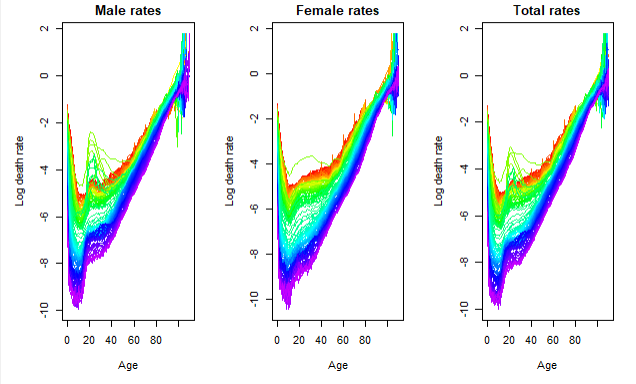
\includegraphics[width=6.5in]{death_rate_par_rapport_age.png}
    \caption{Logarithme de taux de mortalité (1872-2017) en Italie par genre }
    \label{fig:log_death_rate_age}
\end{figure}
Les données sur lesquelles nous travaillons sont celles provenant du site internet \texttt{\href{https://www.mortality.org/}{www.mortality.org}}. Il s'agit de \textit{Human Mortality Database (HMD)}, une base de données qui a été créée pour fournir des données détaillées sur la mortalité pour 47 populations homogènes dans différents pays et régions.
\vskip 0.1in
Dans le cadre de notre projet, nous nous sommes concentrés sur les données concernant l'Italie et qui se présentent comme ceci:
\vskip 0.1in
\begin{itemize}
    \item \textbf{year}: les années pour lesquelles la mortalité a été observée entre \textbf{\textit{1872-2017}}
    \item \textbf{age}: les âges pour lesquelles la mortalité a été observée entre \textbf{\textit{0-110}}
    \item \textbf{pop}: une répartition de la population Italienne selon 3 modalités: année du décès, âge du décès et genre (H/F).
    \item \textbf{rate}: les taux de mortalité observés en Italie repartis selon 3 modalités: année, âge et genre (H/F).
\end{itemize}
\vskip 0.1in

Pour mieux analyser les données, nous commençons par tracer les logarithmes des taux de mortalité de la population Italienne âgée de 0 à 110 ans pour la période 1872-2017 :


\section{Calcul de la Valeur Actuelle Probable  du contrat}
Le problème principal de l’assureur vie est de pouvoir déterminer à la date de souscription d’un contrat quelconque, la valeur d’un engagement à long terme dont la réalisation n’est pas certaine. Pour cela,il utilise la notion de valeur actuelle probable qui combine à la fois la notion de la valeur probable (calcul de probabilité) et celle de valeur actuelle (mathématiques financières).\\
\\
\\
Pour calculer la VAP, plusieurs étapes ont été réalisé.
Nous avons affiché tout d'abord la  table de mortalité qui nous permet de visualiser la probabilité annuel de décès d'un individu et la table actuarielle. Ensuite nous avons calculé la durée de vie attendu afin d'obtenir la valeur actuelle probable.
\\

\\ \textbf{ Étape 1 :} \\
\newline
D'abord ,nous avons converti les taux de mortalité en probabilités de décès
pour la cohorte 1943 à l'aide de la fonction \textbf{mx2qx()} afin de construire la table de survie.\\ 

\newline
\begin{figure}[hhhhhhhh!]
    \centering
    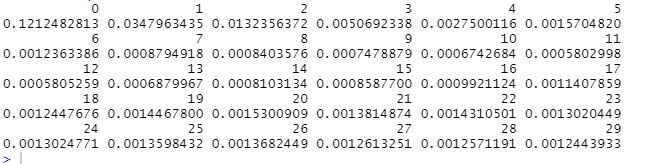
\includegraphics[width=12cm, height=6cm]{kk.png}
    \caption{ La table de mortalité}
\end{figure}
\newline
\\ 
\\ \textbf{ Étape 2 :} \\
\\
Après , nous avons  utilisé la fonction \textbf{probs2lifetable()} pour créer une nouvelle table de survie en précisant la génération de cette table à partir de la probabilité de décès $q_x$ ou de survie $p_x$.
\newline
\newpage
\begin{figure}[hhhhhhhh!]
    \centering
    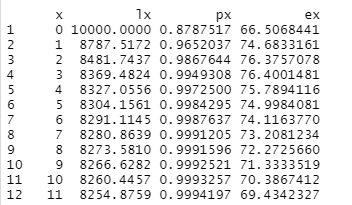
\includegraphics[width=9cm, height=5cm]{9.png}
    \caption{  La table de survie}

\end{figure}


\\ \textbf{ Étape 3 :} \\
\\
Ensuite, nous avons créé une nouvelle table actuarielle qui est générée à partir de la table de survie avec un taux d'intérêt égale à 1.5 \% et qui contient tous les indicateurs nécessaires à l'analyse des résultats par période.
\begin{figure}[hhhhhhhh!]
    \centering
    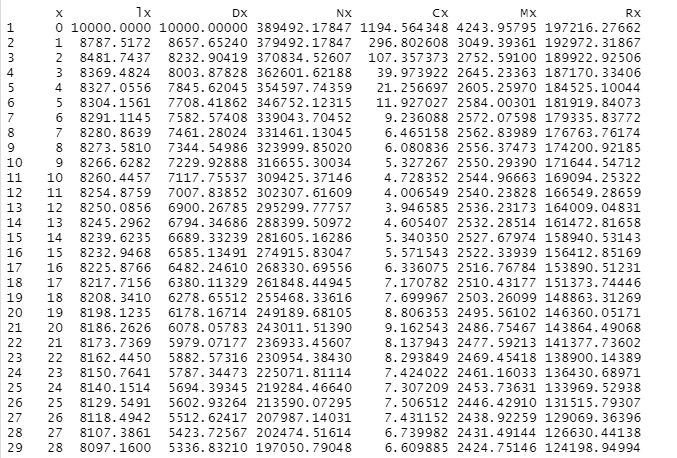
\includegraphics[width=12cm, height=6cm]{8.png}
    \caption{ La table d'actuarielle}
\end{figure}


\\ \textbf{ Étape 4 :} \\

Pour le calcule de la valeur actuelle probable à partir d'un tableau actuariel, nous avons utilisé la fonction \textbf{"axn"} qui permet directement d'afficher le résultat.
\newline
\newline
Le résultat obtenu pour la valeur actuelle probable  pour une cohorte des assurés ayant un contrat en 2015 à l'âge de 40 ans égale à \textbf{0.0001466153 }

\newpage
\section{Calcul de la Valeur Actuelle Probable en utilisant pour mortalité de référence les taux de 2016}
Pour calculer la VAP , plusieurs étapes ont été réalisé.
Nous avons affiché tout d'abord la  table de mortalité qui nous permet de visualiser la probabilité annuel de décès d'un individu et la table actuarielle. Ensuite nous avons calculé la durée de vie attendu afin d'obtenir la valeur actuelle probable.
\newline  

\begin{figure}[hhhhhhhh!]
    \centering
    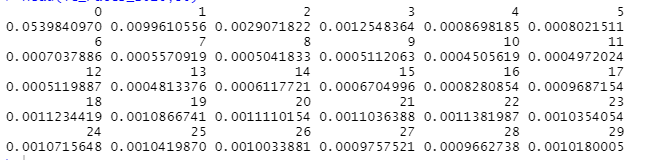
\includegraphics[width=9cm, height=5cm]{mortality_en_proba_de_deces__2016.png}
    \caption{  La table de mortalité en probabilité de decés 2016}
    \label{fig:3.PNG}
\end{figure}
\newline 
\newline 

\begin{figure}[hhhhhhhh!]
    \centering
    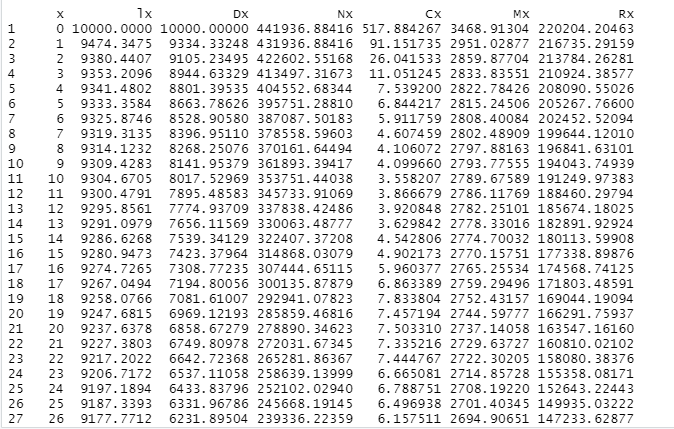
\includegraphics[width=9cm, height=5cm]{table_actuarielle_2016.png}
    \caption{  La table actuarielle 2016}
    \label{fig:3.PNG}
\end{figure}
\newline 
\newline 
Le résultat obtenu pour la valeur actuelle probable  en utilisant pour mortalité de référence les taux de 2016  pour une cohorte des assurés ayant un contrat en 2015 à l'âge de 40 ans égale à \textbf{0.0001248352 }







\section{Extrapolation des taux de mortalité par la méthode de Coale et Kisker}

\subsubsection{Choix de la plage d'âge: Fermeture de tables}
Avant d’utiliser des modèles d’ajustement, il convient de "fermer" les tables, les
taux bruts au delà de 90 ans étant inexploitables. Différentes méthodes existent sur ce point et
nous retiendrons ici la méthode de Coale et Kisker (COALE et KISKER [1990])\cite{Coale et Kisker} qui conduit à
des résultats satisfaisants. Cette méthode consiste à extrapoler les taux instantanés de
mortalité aux grands âges (jusqu’à x = 110 ans par exemple) en se basant sur la formule
\[   g_{x} = \ln (\frac{ \hat \mu_{x}}{\hat \mu_{65}} )/ (x - 65), x\geq 65  \]
Coale et Kisker ont en effet remarqué empiriquement que les courbes des $g_{x}$
possèdent en général un pic aux alentours de 80 ans avant de décroître linéairement. Ils ont
par conséquent proposé l’équation :
\[   g_{x} = g_{80} + s (x- 80), x \geq 80\]
Avec: \\
$s$ le taux de croissance
du taux à partir de 80 ans
 \[   s = - \frac{\ln (\hat \mu_{79} + 31g_{80})}{465}   \]
 et $g_{80}$ représente l’étendue entre le log taux de mortalité à l’âge 65 ans et celui à 80 ans
 \[g_{80}=\frac{\ln(\frac{ \hat \mu_{80}}{\hat \mu_{65}} )}{15}\]
 
 
 A partir de la méthode de Coale et Kisker, nous pouvons affirmé que l'intervalle d'âge va être [80,110]. Puisque avec la fonction $g(x$) nous avons la contrainte que l'âge doit être au delà de 80 ans.
 
 Alors pour ce stade là, nous avons choisi comme âge maximum une valeur qui appartient à l'intervalle [80,110].

 

\section{Estimation des paramètres du Lee Carter}

\subsection{Estimation par le modèle \textbf{lca()}}
Pour s'adapter au modèle Lee-Carter (sans passer par les logarithmes), la fonction \textbf{lca()} (Latent Class Analysis) peut être utilisée. LeeCarter est ici appliqué séparément entre la population masculine, féminine et totale et en considérant un âge maximum appartient à [80,110]. Cette hypothèse sera utilisée pour la calibration dans le  modèle de
mortalité qui sera présenté dans les sections suivantes.\\
\\
\textbf{lca} est un modèle de mesure dans lequel les individus peuvent être classés en types mutuellement exclusifs et exhaustifs, ou classes latentes, en fonction de leur modèle de réponses sur un ensemble de variables indicatrices catégorielles.
\\

\newline--- \textbf{lca()} retourne un objet qui nous permet d'inspecter  ${a}_{x}$, ${{b}}_{x}$ et ${k}_{t}$.
. Les chiffres représentent les valeurs des paramètres estimés.

\begin{figure}[hhhhhhhh!]
    \centering
    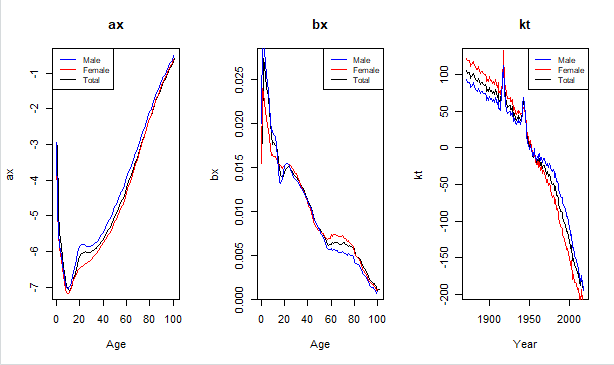
\includegraphics[width=15cm, height=12cm]{lca_function_estimation_parametres.png}
    \caption{Les valeurs estimées des  ${a}_{x}$, ${{b}}_{x}$ et ${k}_{t}$ du modèle}
    \label{fig:lca_estimation.png}
\end{figure}

La Figure \ref{fig:lca_estimation.png}  représente cette estimation à partir des données masculines et féminines italiennes.\\
\newline
Un comportement similaire des paramètres est observé selon différents ensembles de données.\\
\\
Comme prévu la mortalité moyenne augmente lorsque l'âge augmente (voir schéma $\hat{{a}}_{x}$).\\
\\
En outre, il est clairement visible la jeune bosse de mortalité pour les hommes dans la tranche d'âge (20,30) en raison de décès accidentels.\\
\\
Le coefficient estimé $\hat{{b}}_{x}$ montre plutôt une valeur plus élevée pour les jeunes âges et une plus grande amélioration pour la tranche d'âge (60-80).\\
\\
Enfin, comme prévu, $\hat{{k}}_{x}$ a une tendance à la baisse avec l'augmentation de temps.\\
\newline



\subsection{Estimation en utilisant le package StMoMo}

\subsubsection{Package StMoMo}

StMoMo (Stochastic Mortality Modeling) est un package R fournissant des fonctions pour spécifier et ajuster les modèles de mortalité stochastique, y compris les modèles Lee-Carter, le modèle CBD, le modèle APC et de nombreux autres modèles. L'ensemble comprend également des outils pour analyser la qualité de l'ajustement des modèles et effectuer des projections et des simulations de mortalité.\cite{StMoMo}

\subsubsection{Choix de la période choisie}
D'après la première méthode d'estimation des coefficients du modèle Lee Carter ( avec la fonction prédéfinie \textbf{lca()}, nous avons provoqué qu'il faut restituer l'intervalle des années 1872-2017.
\\








Dans la figure \ref{fig:kt.png}, la courbe montre que la valeur de ${k}_{t}$ est presque stable, autour du valeur 100 de l'année 1872 jusqu'à 1900, avant de marquer une forte décroissance.
Ainsi, cette courbe présente deux grands pics de valeur de ${k}_{t}$ qui expliquent que l'italie a participé dans les deux guerres mondiales respectivement en 1914 et 1939.
Alors, nous avons avoué une différence sur les années les plus récentes mais aucune sur les années les plus anciennes. 
Comme nous souhaitons projeter, nous allons restreindre notre étude aux années 1900 - 2017 pour la calibration de modèle de mortalité


\begin{figure}[hhhhhhhh!]
    \centering
    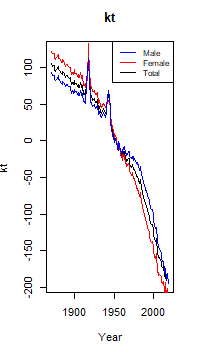
\includegraphics[width=15cm, height=9cm]{visualisation_param_kt.png}
    \caption{Les valeurs estimées de ${k}_{t}$ du modèle avec \textbf{lca()}}
    \label{fig:kt.png}
\end{figure}




\subsubsection{Application de la méthode}
On va estimer différemment les coefficients du modèle Lee Carter avec le package StMoMo en appliquant les étapes suivantes :\\
\newline
\newline
--- Charger les données annuelles disponibles par années d'âge dans la base HMD. \\
\newline
---  Appliquer une fonction qui va créer un objet StMoMoData adapté à l'ajustement d'un modèle de mortalité stochastique.\\
\newline
---Une transformation des données StMoMo des expositions centrales en expositions initiales sera appliquée. Les expositions initiales sont calculées en ajoutant la moitié des décès aux expositions centrales en utilisant la fonction \textbf{central2initial()}. \\
\newline
--- Assumer à avoir un seuil d'âge égale à 100 ans.\\
\newline
--- Génèrer une matrice de poids en fonction d'un groupe d'âge et d'années et d'un ensemble de cohortes étant donné un poids nul. Ceci est utile pour exclure certains points de données lors de l'ajustement d'une mortalité stochastique par la fonction \textbf{genWeightMat()}.\\
Cette dernière comporte un argument à calibrer qui est \textit{clip} qui est le nombre de cohortes dans la limite pour attribuer un poids nul. Cela peut être utilisé pour peser zéro certaines des premières et dernières cohortes dans les données.
Dans l'exemple italien, nous avons pris la valeur de clip égale à 3.\\
\newline
--- Estimer le modèle LC(Lee-Carter)
avec le paramètre link qui  définit la fonction de liaison et la composante aléatoire associées au modèle de mortalité. Nous avons opté pour "log" qui supposerait que les décès suivent une distribution de Poisson et utilisent un lien logarithmique tandis que "logit" supposerait que les décès suivent une distribution binomiale.

\begin{figure}[hhhhhhhh!]
    \centering
    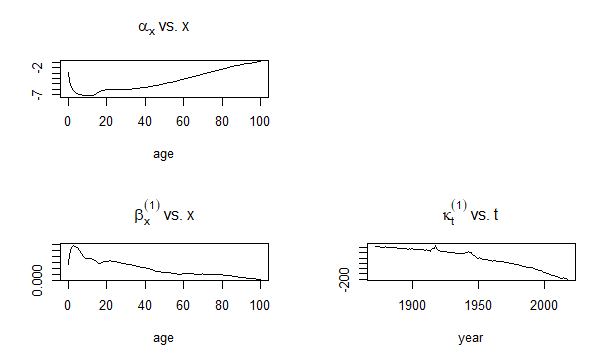
\includegraphics[width=15cm, height=13cm]{estimation_param_avec_stMoMo_fit.png}
    \caption{Les valeurs estimées des  ${a}_{x}$, ${{b}}_{x}$ et ${k}_{t}$ du modèle avec le package StMoMo}
    \label{fig:stmomo_estimation.png}
\end{figure}
\newpage

La figure \ref{fig:stmomo_estimation.png} ci-dessus montre les ajustements LC.
\newline
\\ \textbf{ Étape 1 : Estimation du coefficient $\hat{{a}}_{x}$} \\
La courbe, relativement élevée chez les nouveaux-nés et décroît rapidement avec l’âge pour atteindre son minimum absolu vers l’âge de 10 ans. On survient d’ailleurs un pic de mortalité discrètement appelé "bosse-accident". Cette bosse, qui touche les jeunes d’une vingtaine d’années, est en fait essentiellement composée de deux sortes d'évènements, suicides et accidents. Ensuite, les logarithmes moyens des taux instantanés de mortalité augmentent pratiquement linéairement avec l’âge.
\\ \textbf{ Étape 2 : Estimation du coefficient $\hat{{b}}_{x}$} \\
Les paramètres $\hat{{b}}_{x}$ représentent l’interaction de l’effet des années calendaires sur les taux de mortalité. Cet effet est toujours positif mais la valeur ne cesse de diminuer avec l’âge. Autrement dit, l’effet des années calendaires agit majoritairement avant 60 ans et de moins en moins au delà. On constate une bosse à 22 ans.
Au contraire, vers les âges élevés , $\hat{{b}}_{x}$ avoisine zéro et la chute temporelle de la mortalité est donc beaucoup moins sensible.
\\
\\ \textbf{ Étape 3 : Estimation du coefficient $\hat{{k}}_{x}$} \\
Enfin, comme prévu, $\hat{{k}}_{x}$ a une tendance à la baisse avec l'aide de temps

\section{Projection du taux de mortalité}
\subsection{Le Package Forecast}
Le package contient des méthodes et des outils pour afficher et analyser des prévisions de séries temporelles univariées, y compris le lissage exponentiel via des modèles d'espace d'état et la modélisation automatique \textbf{ARIMA}. \cite{package forecast}


\subsection{Mise en oeuvre avec la méthode forecast}
Il s'agit d'une fonction générique de prévision à partir de séries temporelles ou de modèles de séries temporelles.
\subsubsection{Choix du nombre d'année}
Pour soumettre le forecast,La valeur horizon est mise à 50 ans.

\begin{figure}[hhhhhhhh!]
    \centering
    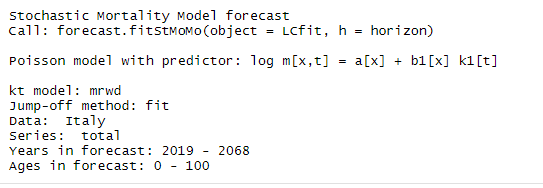
\includegraphics[width=14cm, height=10.5cm]{forecast_details.png}
    \caption{ Détails forecast }
    \label{fig:prediction1.png}
\end{figure}

\subsubsection{Application de la prévision}

Forecast utilise des informations sur les fluctuations de la vitesse du changement dans le passé pour estimer
l'intervalle de confiance pour l'incertitude qui enveloppe le taux de mortalité dans l'avenir.\\ 
\newpage
Les valeurs prévues de ${k_{t}}$ remises à zéro au cours de la dernière année observée (2017) sont rapportées ici.\\
\begin{figure}[hhhhhhhh!]
    \centering
    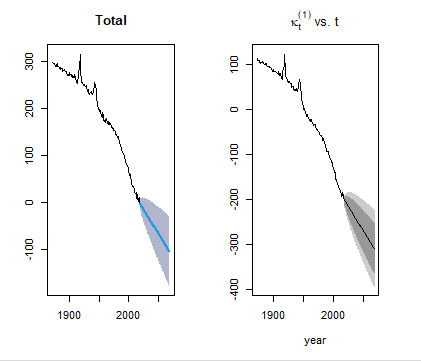
\includegraphics[width=14cm, height=10.5cm]{projection_forecast.png}
    \caption{ Projection du taux de mortalité pour les 50 prochaines années }
    \label{fig:prediction1.png}
\end{figure}

La Figure \ref{fig:prediction1.png}, nous trouvons les intervalles de confiance à 95\% et les comparons avec les estimations du modèle classique
de Lee et Carter. Remarquons que les
taux de mortalité en 2050 générées par le modèle de Lee et Carter se situent dans cet intervalle. Ceci prouve qu’il n'existe pas une différence significative
entre l’ajustement du modèle, du moins pour les données italiennes.

\section{Recalcul de la valeur actuelle probable en utilisant les taux projetés }


Pour recalculer la VAP , plusieurs étapes ont été réalisé. Nous 
avons projeté les taux de mortalité à l’aide de la fonction forecast puis on les a utilisé afin d’obtenir la valeur actuelle probable.
\newline
\newline
\newline
Le résultat obtenu pour la valeur actuelle probable  en utilisant les taux de mortalité projetés égale à \textbf{0.5373275 } qui est largement supérieur a la valeur actuelle probable qu'on a calculer à partir d'une table de mortalité donnée .
\newline
 



\section{Conclusion}
Dans ce dernier chapitre
,nous avons mis en évidence l’influence du taux d’intérêt sur la valeur actuelle probable d’une rente viagère sur les données italiennes.
nous avons définit les différents étapes faites pour atteindre cet objectif.
D'abord, nous avons estimé et projeté le taux de mortalité de la population italienne a l’aide du modèle Lee carter,
ensuite, nous avons calculé la valeur actuelle probable d'une rente viagère a terme anticipé et temporaire  d’une durée de 15 ans, et pour finir nous avons
étudié la variation du taux d’intérêt sur la valeur actuelle probable
et la variation du taux de mortalité sur la valeur du taux d’intérêt.


\chapter*{Conclusion Générale} 
\addcontentsline{toc}{chapter}{Conclusion Générale}


L'objectif de ce projet est  d'estimer  l'impact des taux d'intérêt sur la valeur actuelle probable d'une rente viagère.Pour ce faire, nous avons procéder à une estimation du taux de mortalité de la population Italienne  sur une période s'étalant de 145 ans (1872-2017).
%La moyenne du taux de mortalité observé courant la période s'élève à ..... avec un écart-type de ... .
\vskip 0.1in
Statistiquement, le taux de mortalité a connu une baisse sur la période d'analyse. Nous soulignant toutefois deux pics correspondants aux deux guerres mondiales (1914-1918 et 1941-1946).
\vskip 0.1in
La test d'un modèle stochastique (modèle de Lee-Carter) a permis de quantifier la longévité en deux étapes:
\begin{itemize}
\vskip 0.1in
    \item une première étape consistant à l'estimation des paramètre de ce modèle selon deux modalité différentes: le modèle lca et le package StMoMo. Les résultats de ces estimations ont permis de conclure que la mortalité moyenne augmente avec l'âge avec une nette différence selon le genre pour la tranche d'âge 20-30 qui semble correspondre à des décès qualifiés d'accidentels pour les hommes.
    \vskip 0.1in
    \item Dans une seconde étape, nous avons procéder à une projection des taux de mortalité sur une période de 50 ans. Cette projection a permis de conclure que les taux de mortalités générés par le modèle de Lee-carter restent significatifs à 95\%.
\end{itemize}
\vskip 0.1in
Par ailleurs, pour répondre à la question posée nous avons procédés au calcul de la valeur actuelle probable pour la cohorte 1943 et ce:
\vskip 0.1in
\begin{itemize}
    \item Pour une rente viagère à terme anticipée estimée à 11.21
    \vskip 0.1in
    \item Pour une rente viagère temporaire d'une durée de 15 ans estimée à 0.63
\end{itemize}
\vskip 0.1in
De plus, l'estimation de la variation de la valeur actuelle probable en fonction des taux d'intérêt a permis de conclure l'existence d'une relation inverse entre ces dernières: La valeur actuelle probable aura tendance a baisser quand le taux d'intérêt augmente.
\vskip 0.1in
Enfin, l'étude de la variation du taux d'intérêt en fonction de taux de mortalité montre que ce dernier baisse quand le taux d'intérêt augmente.
\vskip 0.1in
Il est ainsi possible d'infirmer que pour la gestion des contrats d'assurance vie, la sous estimation des taux de mortalité engendrera une réduction des prestations en valeur actuelle probable et donc taux d'intérêt plus important.

%\addcontentsline{toc}{chapter}{Références}

%https://www.ssa.gov/oact/NOTES/as116/as116_IV.html
%https://www.capital.fr/votre-argent/capital-deces-1326438
%http://www.dicodunet.com/definitions/economie/rente-temporaire.html
%https://www.journaldunet.fr/business/dictionnaire-economique-et-financier/1198837-valeur-actuelle-definition-calcul-traduction/
%https://www.lafinancepourtous.com/pratique/retraite/epargne-retraite/la-rente-viagere/
%https://epatrimoine.fr/definition-assurance-vie\pagestyle{}

%\newline
%https://cran.r-project.org/doc/contrib/Charpentier_Dutang_actuariat_avec_R.pdf?fbclid=IwAR3CBOpQj6rsPjlltyPbwqinQazYjqAI57npvsq8NRx3o-896aMz8dylnUM

%http://dictionnaire.sensagent.leparisien.fr/M%C3%A9thode%20des%20moindres%20carr%C3%A9s/fr-fr/

%https://www.rdocumentation.org/packages/StMoMo/versions/0.4.1

%http://www.ressources-actuarielles.net/EXT/IA/sitebfa.nsf/0/F996B9C58C812708C1257396004BB743/$FILE/PLANCHET_LELIEUR.pdf?OpenElement

%https://cran.r-project.org/web/packages/forecast/forecast.pdf

\addcontentsline{toc}{chapter}{Bibliographie}
\begin{thebibliography}{9}



\bibitem{Max de vraisemblance1}
Charpentier, A. Dutang, C. (2012). \textit{Actuariat Avec R}. \texttt{\url{https://cran.r-project.org/doc/contrib/Charpentier_Dutang_actuariat_avec_R.pdf}}
\vskip 0.1in

\bibitem{Max de vraisemblance2}
Dagnelie, P. (2007), \textit{Statistique théorique et appliquée}
De Boeck Université. 21
\vskip 0.1in

\bibitem{Max de vraisemblance3}
Dalgaard, P. (2008), \textit{Introductory Statistics with R}
Springer. 21
\vskip 0.1in

\bibitem{Max de vraisemblance4}
Hogg, R. V., Craig, A. T. \& McKean, J. W. (2005),
\textit{Introduction to Mathematical Statistics}, 
6edn, Prentice Hall, Upper Saddle River, NJ. 21
\vskip 0.1in


\bibitem{Max de vraisemblance5}
Saporta, G. (2006), 
\textit{Probabilités, analyse de donnés et statistique}
Technip. 21, 29
\vskip 0.1in


\bibitem{Lee Carter}
VU Tuan Anh, \textit{Modèle Lee Carter}. \texttt{\url{https://www.institutdesactuaires.com/}}
\vskip 0.1in


\bibitem{Moindre carree}
\textit{Méthode des moindres carrés}. Consultée sur \texttt{\url{http://dictionnaire.sensagent.leparisien.fr/M\%C3\%A9thode\%20des\%20moindres\%20carr\%C3\%A9s/fr-fr/}}
\vskip 0.1in

\bibitem{Estimation modele Lee Carter}
Antoine Delwarde (2003-2004). \textit{Modèle log-bilinéaire pour
l'élaboration de tables de
mortalité prospectives}. \texttt{\url{https://www.scor.com/fr}}
\vskip 0.1in


\bibitem{VAP}
Jakubowicz, L. (2019), \textit{Valeur actuelle : définition, calcul, traduction}. La rédaction JDN, consultée sur \texttt{\url{https://www.journaldunet.fr/business/dictionnaire-economique-et-financier/1198837-valeur-actuelle-definition-calcul-traduction/}}


\vskip 0.1in
\bibitem{renteV}
La Finance Pour Tous, (2019). \textit{La rente viagère}. Consulté sur \texttt{\url{https://www.lafinancepourtous.com/pratique/retraite/epargne-retraite/la-rente-viagere/}}
\vskip 0.1in

\bibitem{Cours}
 Maatoussi, & Anis, (2019-2020). \textit{Cours actuariat vie 2019-2020}. 
\vskip 0.1in

\bibitem{rente temporaire}
Dico Du Net, \textit{Rente temporaire}. Consulté sur \texttt{\url{http://www.dicodunet.com/definitions/economie/rente-temporaire.htm}}
\vskip 0.1in

\bibitem{mortalite}
Felicitie C. Bell et Michael L. Miller. \textit{Life Tables for the United States Social Security Area 1900-2100}. Consulté sur \texttt{\url{https://www.ssa.gov/oact/NOTES/as116/as116_IV.html}}
\vskip 0.1in

\vskip 0.1in
\bibitem{Coale et Kisker}
UTILISATION DES METHODES DE LEE-CARTER ET LOGPOISSON POUR L'AJUSTEMENT DE TABLES DE MORTALITE
DANS LE CAS DE PETITS ECHANTILLONS, \textit{Méthode de Coale et Kisker}. Consultée sur \texttt{\url{http://www.ressources-actuarielles.net/}}
\vskip 0.1in


\bibitem{StMoMo}
Villegas, A., Kaishev, V. K., \& Millossovich, P. (2015). \textit{StMoMo: An R package for stochastic mortality modelling}. In 7th Australasian Actuarial Education and Research Symposium. \texttt{\url{https://cran.r-project.org/web/packages/StMoMo/vignettes/StMoMoVignette.pdf}}
\vskip 0.1in


\bibitem{package forecast}
Hyndman, R. J., Athanasopoulos, G., Bergmeir, C., Caceres, G., Chhay, L., O'Hara-Wild, M., ... & Wang, E. (2020). \textit{Forecasting Functions for Time Series and Linear Models}. \texttt{\url{https://cran.r-project.org/web/packages/forecast/forecast.pdf}}.
\vskip 0.1in









\end{thebibliography}
\end{document}